\section{Introduction}
\label{sec:introduction}

\subsection{Background}

\ToDo{1 Cyber attacks are diversifying.}

\ToDo{2 Threat intelligence and threat reports are helpful tools}

Provenance graph as a threat representation tool are already widely studied and adopted \cite{li2021}. With provenance graph, security analyzers are able to encode system execution history into graphs. Thus provenance graph contain rich semantic information. However, there are still a gap between provenance graphs and human understandable information. Poirot \cite{Milajerdi2019} try to solve this problem by involve TTPs and kill chain proposed by MITRE \cite{}.

\ToDo{3 Provenance graph are widely-used and recongnized threat representation approach.}

\subsection{Related Works}

\ToDo{1 Compare with existing automated threat intelligence collection works.}

\ToDo{2 How our work support provenance graph-based threat detection.}

\subsection{Our work}

\ToDo{1 Extracting incomplete attack graph from single CTI report.}

\ToDo{2 Delineating behavioural and clustering analysis.}

\ToDo{3 Implement applicaitons.}

\subsection{Contribution}

\ToDo{1 New threat intelligence representation approach.}

\ToDo{2 Automated threat intelligence collection and management system.}

\ToDo{3 Collected a large amount of threat intelligence and done a through analysis by real-word application.}

\ToDo{4 We provided a open attack dataset.}


\begin{figure}
    \centering
    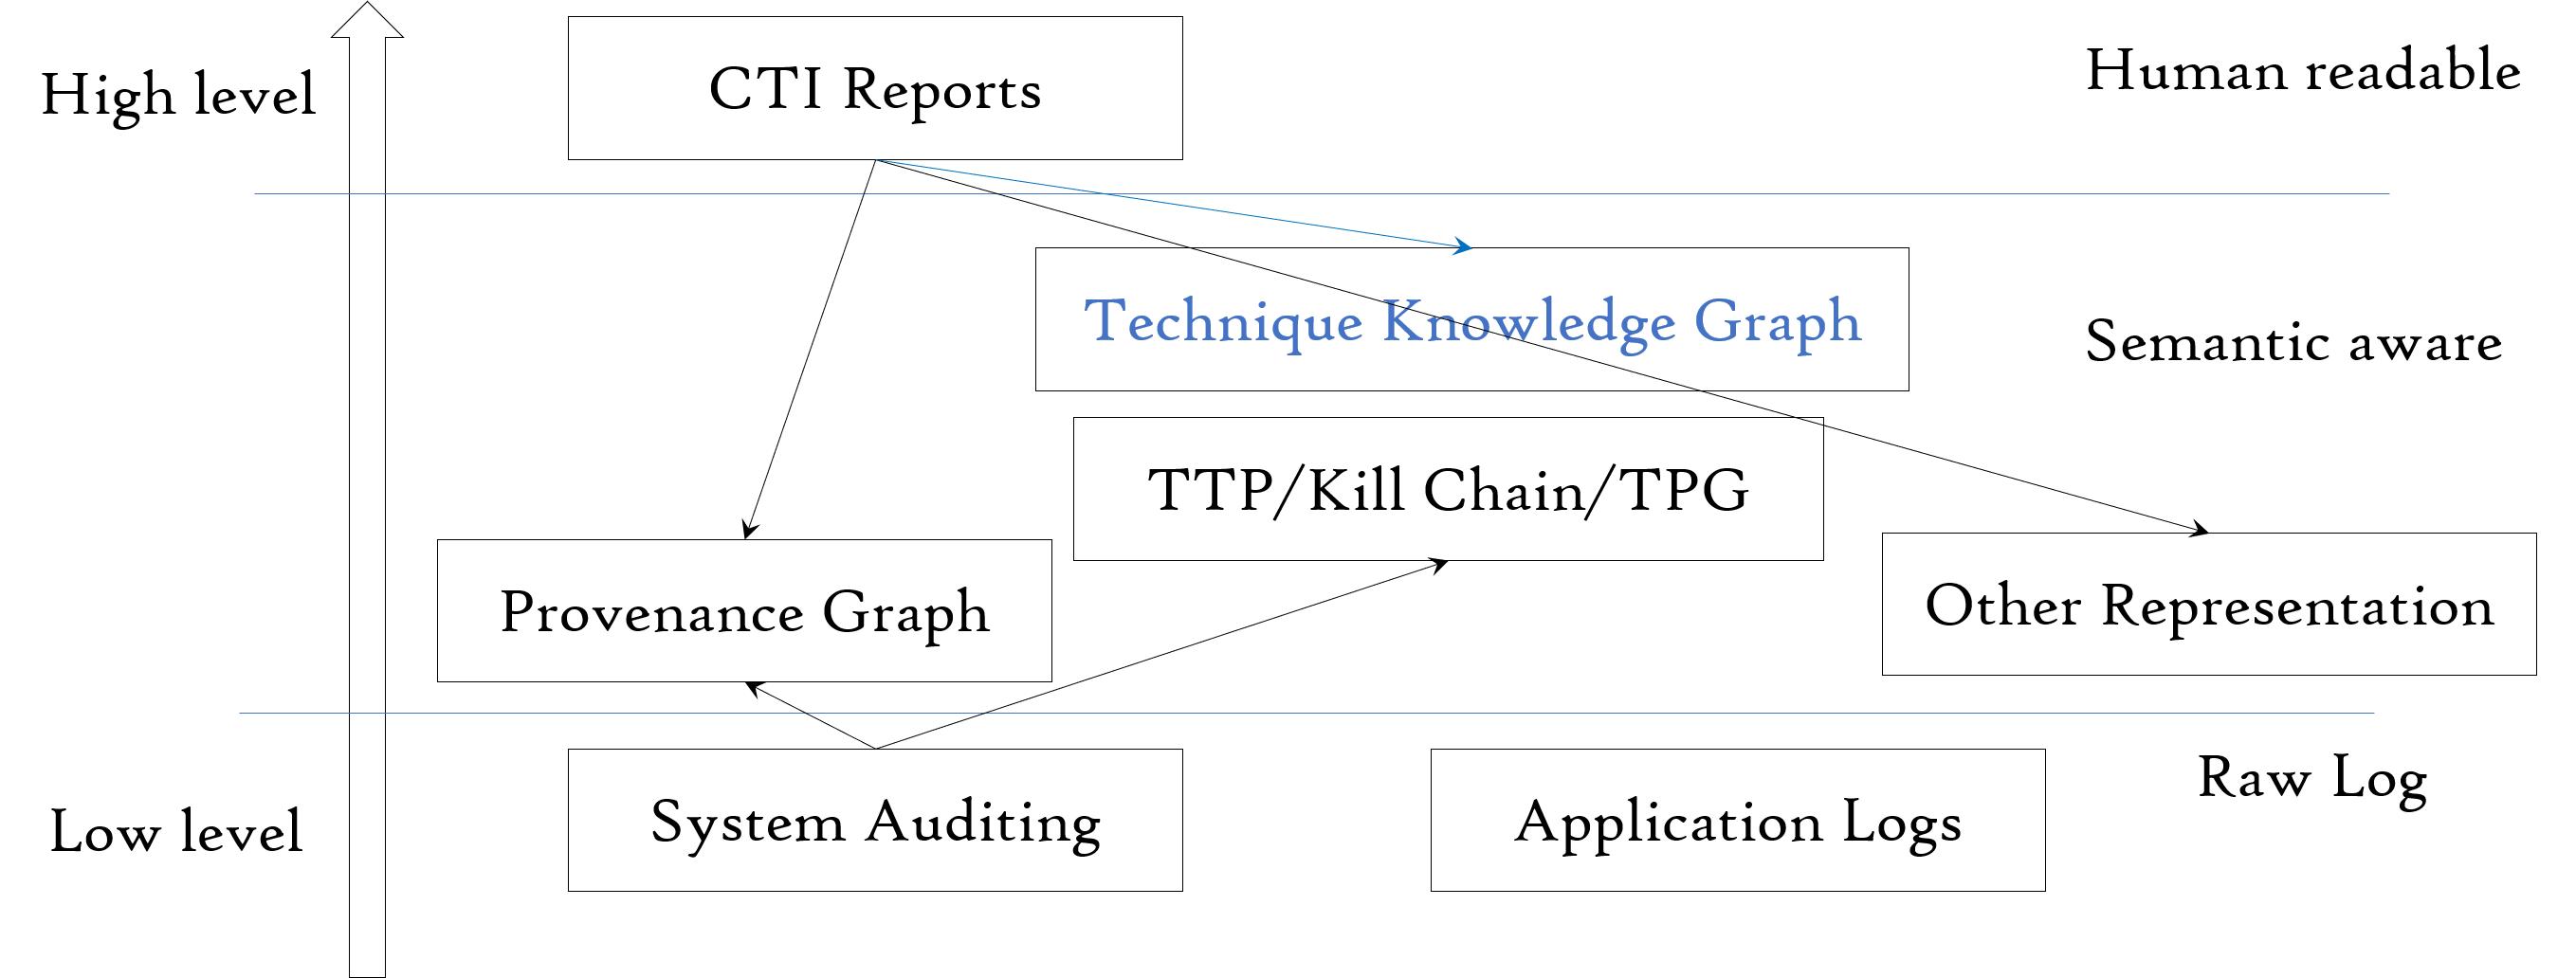
\includegraphics[width=3.5in]{Image/representation.png}
    \caption{Different Representation of Cyber Attacks.}
    \label{fig:representation}
\end{figure}
